\chapterauthor{Jay Lofstead}{Sandia National Laboratories}
\chapterauthor{Eric Barton}{Intel}
\chapterauthor{Matthew Curry}{Sandia National Laboratories}
\chapterauthor{Carlos Maltzahn}{University of California, Santa Cruz}
\chapterauthor{Robert Ross}{Argonne National Laboratory}
\chapterauthor{Craig Ulmer}{Sandia National Laboratories}

\chapter{The Convergence of Enterprise, Internet Scale, and High Performance
             Computing Storage Infrastructures}

\section*{Abstract}
Large scale storage infrastructures have been significantly impacted by the
growth in data analytics applications. High Performance Computing storage
infrastructures, once the extreme end of the storage scale spectrum, must now
adapt to technologies optimized for large scale data analytics applications.
Hardware changes, such as storage class memory, are also affecting how
the exascale storage stack will be constructed. We examine use cases, trends,
convergent technologies, and new opportunities generated by this technology
blending.

\section{Introduction}\label{sec:intro}
HPC infrastructures have grown around the requirement to handle large,
decomposed data structures for parallel computation. Single data objects may be
hundreds of terabytes spread across an entire machine. Parallel storage systems
have grown trying to address performance and storage requirements while
maintaining backwards compatibility with the standard POSIX interface and
semantics.  Unfortunately, this is proving increasingly difficult, as the POSIX
specification was not designed to efficiently support parallel
storage~\cite{kimpe:2014:storagemodels}.

Big data and internet-scale applications, on the other hand, focus on searching
through immense volumes of small, loosely associated items looking for patterns
or correlations that may lead to insights. Some science applications, such as
genomics, have a workload pattern similar to these big data
applications. Parallel file systems are not well suited to these workloads
because the broad, relatively continuous read demand of independent items does
not benefit from the coordination overheads of parallel file systems. Instead,
distributing loosely coordinated storage across the compute infrastructure makes
more sense. With pressures to effectively leverage a single platform for these
disparate workloads and the shifting storage market, new considerations for how
to design storage resources for extreme scale compute systems must be made.

Traditionally, the HPC market has focused on supporting coherent and consistent
output methods from parallel sources to parallel targets. This requirement is
driven from validating that the output of a single item is complete and
correct. Largely, the workload is write-intensive during the expensive, at scale
computation process with a read-intensive phase lasting months on cheaper
machines or at small scale with low priority. File systems like the dominant
Lustre~\cite{braam:2002:lustre-arch} and GPFS~\cite{schmuck:2002:gpfs} systems
have been carefully optimized to address these workloads.

The big data market has opposite priorities. The big computation phase requires
reading large quantities of data for processing at scale. The output from this
process can be handled at much smaller scale later and is orders of magnitude
smaller. Given the read-dominant focus, the overhead inherent in coherent and
consistent storage for write intensive workloads is both unnecessary and a heavy
cost. Instead, systems like HDFS~\cite{shvachko:2010:hdfs} dominate.  These work
by storing files that will be read for processing throughout the compute area,
including the assumption that storage failures are common, prompting
replication.

The output from initial stream or file processing for the big data workloads use
distributed object-based storage technology. It offers independent,
uncoordinated data access with a simplistic key search space for subsequent
analysis. The profit potential for this market has caused an explosion in
specialized products aimed at accelerating this processing style.  For small
enough data sets, in memory object stores like memcached and Radius dominate.
For larger data sets, approaches like Google's Big Table are accomplishing the
same function. There are also hardware products targeting this market segment,
such as Kinetic~\cite{segate-kinetic}, offering a native object interface for
the devices connected directly to a network.

Adding complexity to this storage environment is the relentless performance
improvements and cost reductions for solid state storage, like NAND-based flash
memory. These devices have already rendered 15,000 RPM disk drives obsolete.
The 10,000 RPM disk drives will not survive for more than a few more years.
New disk technology like shingled drives~\cite{wood:2009:shingled-media} offer
a path for disks to survive longer. The enormous capacities for read intensive,
write infrequently workloads is very attractive for many communities. For
example, storing images created sequentially for later read-intensive
processing can yield a better cost/performance balance.

This chapter investigates these new technologies and how they affect extreme
scale computing. We evaluate how the HPC environment can and must adapt to this
new storage environment to address future computing needs and to take advantage
of the different kinds of technology being developed. We will also consider the
planned reintegration of large scale computing from the split of big data
applications from simulation-based computing with both the necessary and forced
integration of these large, expensive platforms for multi-use.

\section{Existing File Systems}

HDFS developed to support the Hadoop implementation of the MapReduce system. It
offers a distributed, replicated file store optimized to support the MapReduce
processing configuration. Ceph also addresses this distributed computing
infrastructure, but with a different emphasis. It seeks to offer scale out
performance for objects across a storage infrastructure. However, Ceph does not
offer the ability to scale up: Each object must fit within a single storage
device. With the rise of cloud systems using object-based storage, such as
Amazon's S3, the interaction style offered by Ceph has been adopted for similar
workloads. Ceph has features to handle storage devices failing and new ones
joining a running system without interruption. Ceph offers a complete file
system including metadata management support as well as an object system for
users. GlusterFS focuses on providing a network attached storage interface to
storage distributed throughout a cluster. Rather than providing metadata
services, GlusterFS relies on the underlying storage file system for most basic
capabilities, such as security.

Parallel file systems are optimized to support large files that must be spread
across multiple devices. For example, a 100~TB file cannot fit on any current
storage device and cannot be stored with any performance. Parallel file systems
solve this problem by using multiple devices spread across multiple servers
together as if they are a single device. Data is striped across devices, all of
which can be written to or read from simultaneously. This parallel access
offers aggregate performance enabling manipulating very large files with
reasonable performance. Because of these characteristics, parallel file systems
are deployed on most simulation intensive large scale compute systems to handle
the large single object output characteristic of these applications.  Lustre is
arguably the most popular parallel file system appearing on a majority of the
Top500 machines. IBM's GPFS is increasing in popularity as optimizations
focusing on addressing big data workloads are incorporated. PVFS offers a
rethinking of some of Lustre's earlier limitations to give better scalability
characteristics.

~\\
\noindent\textbf{Discussion}\\
The different optimizations distributed vs. parallel file systems offer are at
the cost of supporting the other kind of workload. As was mentioned above,
parallel file systems aim to support very large objects and aggregate
simultaneous writing and reading for a single object across the array. For
workloads consisting of entirely small objects, this functionality and overhead
is a cost. Similarly, the inability of the distributed file systems to handle
arbitrarily large objects and massive parallel simultaneous access to a single
object make them unsuitable for simulation workloads.

For both workloads, a more flexible object-based interface are being
considered. This is discussed more below.

\section{Object-Based Stores}\label{sec:intro}

The earliest object store is probably the Wisconsin Storage
System~\cite{1985:chou:wisconsin-storage} published in 1985. It offered a
general storage infrastructure for both databases and file systems. Many
current systems were built using a similar infrastructure, such as
Lustre~\cite{braam:2002:lustre-arch}, GPFS~\cite{schmuck:2002:gpfs}, and
Panasas~\cite{welch:2008:panasas}. The general idea is to offer s a
standardized way to address an arbitrary storage space with a key-based access.
These object storage systems assume that some sort of structure is imposed on
top to track what objects correspond to which user items.

While object storage may have been used behind the scenes for years, raw
object storage exposed to the end-user programmer did not into vogue until the
big data era arrived. System developers for big data processing realized that
the overhead imposed by the object management forced serialized or at least
coordinated access. By shifting the mapping load to the end-user programmer
level and using the object storage layer directly, greater perceived
performance can be achieved. In many cases, by stripping down the requirements
to the absolute minimum required semantics for a particular application,
actual performance gains are achieved. The explosion of specialized storage
systems like HDFS and GFS represent this model. Key for this model achieving
performance is the ability of each process to work independently without any
required consistency or coherence with neighbor processes potentially working
on part of the same data set. The dominant object stores are systems like
Memcached~\cite{fitzpatrick:2004:memcached}. This stands in stark contrast to
how supercomputing applications generally operate.

The supercomputing domain maintained the consistency requirements due to the
bulk synchronous parallel processing. Instead, parallel, that is coordinated,
file systems were embraced. The challenge today is that parallel file systems
are having difficulty effectively scaling to handle the IO demands.

Here we want to talk about how object-based key-value stores are used for big
data applications summarizing the specific features that identify this market
segment.

\subsection{HPC Oriented Object Stores}

Parallel file systems inherently have an object-like layer beneath the surface.
The requirement to spread a single file across multiple devices for capacity
reasons alone prompts this approach. The actual implementation may vary, such
as using individual files within a local file system, each representing part
of parallel file. Popular examples include
Lustre~\cite{braam:2002:lustre-arch} and GPFS~\cite{schmuck:2002:gpfs}.

In some cases, directly using a key-value store for HPC applications is being
considered~\cite{yin:2014:key-value-parallel}. The next generation Lustre
project is also considering a key-value infrastructure~\cite{barton:2013:lustre}
to address performance challenges.

The real challenge with key-value stores for HPC applications is the metadata
management. All of these projects have taken a similar step to the big data
application is that the applications are required to manage the object list to
determine what data is stored in which object.

\section{Next Generation HPC Storage Systems}\label{sec:intro}

Here we want to talk about, at a proposal sort of level, what we think needs
to be done.

Talk about the disconnect between metadata and storage and the complications
it introduces and some ideas on what we plan to do about it.

Talk about the major efforts

\subsection{Lustre/DAOS}

The FFSIO phase II sort of info to start. Keep it acceptable. This seems to me
to be just a pure object store.

\subsection{Kelpie/Data Warehousing}

Kelpie is a distributed, in-memory object store from Sandia National Laboratories that serves as a building block in high-performance computing for implementing custom, data-management services. The fundamental goal of Kelpie is to provide a way for users to decompose their complex datasets into data objects that the library can move between nodes in a safe but efficient manner. Kelpie provides simple abstractions for dealing with distributed data, and utilizes the Nessie communication library to orchestrate how data migrates between nodes. Nessie provides (1) a low-level RDMA layer that has been ported to different HPC fabrics and (2) an RPC layer that enables users to invoke function calls and initiate RDMA transfers on remote nodes. Kelpie uses the former to make an application's data objects accessible by the network interface, and the latter to cooridinate data handoffs between nodes.

Kelpie manages data objects for applications, where a data object is a simply a contiguous block of application data that is labeled with a globally-unique key. The contiguous constraint is necessary because Kelpie registers the memory with the network interface, which in turn allows the hardware to RDMA the data without involving the kernel in virtual to physical address translation. The key used to label an object has three components: an application-specific identifier and a two-dimensional user label. The application-specific identifier enables higher-level services to house different datasets in Kelpie with isolation. Users are not required to use the second dimension of the user label portion of the key. However, the second dimension is often useful for grouping related items together in the store. For example when storing complex mesh datasets in Kelpie, the first dimension of the key (or row) may be used to describe a particular region of a mesh. The second dimension of the key can therefore be used to organize different variables associated with the region (e.g., node locations, pressure, or temperature). This approach allows each variable's data to be stored in its own, independent block of contiguous memory, and provides an opportunity for a user to easily downselect the items they need when retrieving data from Kelpie.

Kelpie nodes are equipped with a Local Key/Value (LKV) structure for managing data objects that are available in the local node. The LKV performs three important tasks. First the LKV provides a means of tracking data objects that are currently in transit and protect the system from deallocating an object before remote nodes have finished transferring it. Second, the LKV structure provides a means for data to be staged at a remote node with only trivial involvement from the destination. For example, an application may push multiple data objects to a node in anticipation of work that will be scheduled on the remote node at a future time. Finally, the LKV structure provides a location for applications to store callbacks to execute when data does arrive at a node. These callbacks make the data store more active and are fundamental to applications that are highly asynchronous or event driven.

In order to address scalability concerns, data management services for HPC typically decompose their work in a hierarchical manner that maps owenership of different portions of the dataset to different groups of nodes that are close in proximity. Kelpie provides the ability to assemble multiple teams of nodes together through a resource management interface. This interface allows users to create and reference a team of nodes together to function as a single data resource that employs a standard data API. A resource has three components: a path-like name that allows a resource to be globally referenced and located by the runtime, a list of physical nodes that implement the resource, and client-side software that defines that policy for how data is managed in the resource. Kelpie provides common implementations of resources, but is easily extended with user-defined modules. A distributed hash table (DHT) is an example of a commonly-used resource in Kelpie. A DHT is composed of N Kelpie servers where data is distributed by using a hash of the first dimension of the key to specify which node should store the object. The DHT resource client software simply maintains the list of servers and then references the proper destination when a user performs put or get operations. Users with reliability concerns have made similar resources just by creating new client software that stores a data object to the hashed server, and a replicated copy to its neighbor. While resources may contain API extensions to support higher levels of functionality, they all support basic communication primitives that enable users to swap one type of resource in for another in most cases.

An example of how Kelpie is being utilized to support data management for higher-level applications can be found in Sandia's DARMA project. DARMA is developing an asynchronous, many-task (AMT) approach to computing that will help codes scale to next-generation platforms. AMT codes specify their execution in the form of a large, directed acyclic graph of tasks (or task DAG) that can be scheduled by a runtime on distributed resources. The data objects consumed and produced by each task form a dependency graph that dictate when and where work can be scheduled. By utilizing Kelpie as the mechanism by which data objects are migrated between different nodes and resources in the system, DARMA can focus on the complex job of making policy decisions about how the work should be orchestrated in the platform.



\subsection{Hybrid Models}

SSIO project from ORNL/Sandia

\section{Conclusions}\label{sec:intro}

This is our overall view on things

\section*{Acknowledgements}
Sandia National Laboratories is a multi-program laboratory managed and operated
by Sandia Corporation, a wholly owned subsidiary of Lockheed Martin
Corporation, for the U.S. Department of Energy's National Nuclear Security
Administration under contract DE-AC04-94AL85000.

%\begin{figure}[htb]
%\begin{figure}[b!]
%\centerline{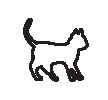
\includegraphics[width=150pt, height=150pt]{Chapters/chapter1/figures/cat.eps}}
%\caption[List of figure caption goes here]{Figure caption goes here. Figure caption goes here.}
%\end{figure}

%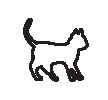
\includegraphics[width=\textwidth]{Chapters/chapter1/figures/cat.eps}
%\caption[Short figure caption]{Figure caption goes here.
%Figure caption goes here.
%Figure caption goes here.}
%\end{figure}

%\section{Glossary}
%\begin{Glossary}
%\item[Adaptable] An adaptable process is designed to maintain effectiveness and
%efficiency as requirements change. The process is deemed adaptable when there
%is agreement among suppliers, owners, and customers that the process will meet
%requirements throughout the strategic period.
%\end{Glossary}

